% AI-MD final report working draft.
% Target: 9 pages in NeurIPS 2025 format.
% All numerical claims below were taken from project artifacts or code.
% REVISION PASS 2026-07-16: every numerical claim was re-verified against the
% source artifacts; all fixes are marked in red (\rev{new text}, \del{deleted text}).
% UPDATE 2026-07-16 (post hybrid judge): the hybrid alpha-sweep set-judge
% (run_r2_judge_hybrid.sbatch) COMPLETED for all 5 folds (parse rate 1.000). It
% OVERTURNED the provisional semantic-only selection: the fused alpha=0.25
% (semantic-weighted) retriever with a top-3 budget wins the label-free selection
% at informative rate 0.327 vs 0.307 for semantic top-5 -- the sole candidate
% inside the 0.005 tolerance band (next best 0.316). Final R2 = L0_CORE /
% hybrid_a25 / top-3. Retrieval-side text below is updated to this outcome.
% The R2 DOWNSTREAM prediction numbers (encoder / LLM / cascade) are being
% recomputed on the new fused evidence (encoder OOF done; Qwen L1-L5 array still
% running); per the experiment rule we do NOT reuse the superseded semantic-R2
% downstream numbers, so Table~\ref{tab:r2} and its prose are marked pending
% refresh (\todoRtwo) until the hybrid-R2 evals complete.
% STILL MISSING FROM THE REPO (compile blockers): neurips_2025.sty and the three
% final vector figures; interim PNG fallbacks from outputs/figures/ are wired in
% below so the draft renders with real content. references_working_v2.bib is now
% provided (two entries flagged for verification).

\documentclass{article}
\usepackage[preprint]{neurips_2025}
\usepackage[utf8]{inputenc}
\usepackage[T1]{fontenc}
\usepackage{hyperref}
\usepackage{url}
\usepackage{booktabs}
\usepackage{amsmath,amssymb,amsfonts}
\usepackage{nicefrac}
\usepackage{microtype}
\usepackage{xcolor}
\usepackage{graphicx}
\usepackage{tabularx}
\usepackage{array}
\usepackage{placeins}
\usepackage{multirow}
\usepackage[normalem]{ulem} % for \del strikethrough revision marks

\graphicspath{{figures/}{outputs/final_report_figures/}{outputs/figures/}}
\newcommand{\todoRtwo}[1]{\textcolor{red}{\textbf{[R2 TODO: #1]}}}
% Revision marks (2026-07-16 review pass): red = changed/added, red strikeout = removed.
% DeclareRobustCommand so the marks survive inside captions (moving arguments).
\DeclareRobustCommand{\rev}[1]{\textcolor{red}{#1}}
\DeclareRobustCommand{\del}[1]{\textcolor{red}{\sout{#1}}}
\newcommand{\best}[1]{\textbf{#1}}
\newcolumntype{Y}{>{\raggedright\arraybackslash}X}

\title{Evidence Selection and Severity Reasoning for PHQ-8 Item-Level Prediction from Mental-Health Interviews}

\author{%
  Daniel Schmidt\thanks{BMIF 203 / BMI 702: AI in Medicine II (AI-MD).}
  \And
  Yaniv Pevzner
}

\begin{document}
\maketitle

\begin{abstract}
Most automated depression-assessment systems predict a binary diagnosis or a single questionnaire total, obscuring the symptom profile that produced that score. We study the harder task of predicting each of the eight PHQ-8 item severities, on an ordinal scale from 0 to 3, from E-DAIC interview transcripts. The resulting dataset contains 219 participants and 1,752 participant--item examples. We decompose the task into two coupled problems: selecting item-relevant evidence from a long interview and inferring ordinal severity from that evidence. A participant-local hybrid retriever combines BM25 with dense semantic similarity, while a MentalBERT encoder with a CORN ordinal head provides a conservative discriminative baseline. A controlled comparison with Qwen2.5-7B-Instruct shows that explicit language-model reasoning recovers substantially more severe cases, but also produces more large ordinal errors. Self-consistency exposes item-level uncertainty, enabling a selective cascade in which an encoder corrects uncertain LLM predictions. The best pre-R2 cascade reaches macro-F1 0.409, QWK 0.447, and MAE 0.606 in participant-grouped out-of-fold evaluation. A subsequent evidence-quality study shows that lexical coverage strongly overestimates usable evidence and that dropping training pairs judged to contain no symptom evidence improves the encoder to macro-F1 0.393, QWK 0.421, and MAE 0.645\rev{, although the later constrained selection rejects this policy on safety grounds}. \rev{A final systematic retrieval study (R2), using a provenance-audited lexicon, natural-language multi-query semantic retrieval, and constraint-based label-free selection, is largely corrective on the retrieval side: lexicon expansion never improves judged evidence quality, and the frozen core vocabulary maximizes it. A judged fusion sweep then shows that calibrated BM25--dense combination---not term expansion---is the best evidence selector: the semantic-weighted ($\alpha=0.25$) retriever with a three-window budget attains judged informative rate 0.327 versus 0.307 for semantic-only retrieval, and is selected as R2. The downstream re-evaluation of the encoder, LLM, and selective cascade on this fused evidence is in progress; the frozen R0 merged-gate cascade (macro-F1 0.409, QWK 0.447, MAE 0.606) remains the reference system pending that refresh.}
\end{abstract}

\section{Introduction}
\label{sec:introduction}
The Patient Health Questionnaire-8 (PHQ-8) summarizes eight depressive symptoms by assigning each item a frequency score from 0 to 3 and summing the items to a total from 0 to 24 \cite{kroenke2009phq8}. Although the total is useful as a compact severity measure, identical totals may arise from different symptom profiles. One participant may primarily report sleep and energy difficulties, whereas another may report depressed mood, anhedonia, and feelings of failure. Recovering the item profile can therefore preserve clinically meaningful structure that is lost when only the aggregate score is predicted.

Predicting item scores from a semi-structured interview is substantially harder than completing the questionnaire directly. Evidence for a symptom may be brief, indirect, distributed across the conversation, or absent from the transcript even when the participant endorsed the corresponding questionnaire item. We therefore view the task as the composition of two distinct problems. First, an evidence-selection mechanism must identify the transcript regions relevant to a particular PHQ-8 item. Second, an inference mechanism must map the selected evidence to an ordinal severity level. Improvements in one component need not improve the other: a richer retrieval query may add irrelevant context, while a more expressive reasoning model may infer unsupported symptoms from general distress.

We investigate this decomposition on E-DAIC interviews using a text-only, participant-local pipeline. Each PHQ-8 item acts as a query over one participant's transcript. Retrieved windows are passed either to a domain-adapted ordinal encoder or to a frozen instruction-tuned LLM. We then analyze whether their different error profiles can be exploited through selective correction, and whether explicit evidence-quality judgments improve training and retrieval selection. All main comparisons use participant-grouped out-of-fold (OOF) evaluation; retrieved text is treated as candidate evidence rather than as a validated clinical rationale.

Our contributions are threefold. First, we formulate PHQ-8 prediction as 1,752 participant--item ordinal decisions and evaluate item-conditioned lexical, semantic, and hybrid retrieval under leakage-safe participant grouping. Second, we isolate the severity-reasoning bottleneck through controlled encoder--LLM comparisons on matched evidence, including cross-item prompting, self-consistency, and confidence-gated correction. Third, we introduce a four-way evidence-quality analysis that distinguishes supporting, opposing, ambiguous, and missing evidence, and use it to study query expansion and missing-evidence training policies. The final systematic retrieval experiment, denoted R2, is designed to determine whether the previous hybrid design is genuinely justified by judged evidence quality rather than inherited configuration choices.

\section{Background and Related Work}
\label{sec:background}
DAIC-WOZ and E-DAIC provide semi-structured interviews and depression-related labels for computational mental-health research \cite{gratch2014daic,devault2014simsensei,ringeval2019avec}. Most prior systems predict depression status or an aggregate PHQ score, often from multimodal audio, visual, and linguistic features. Our target is different: each PHQ-8 item is predicted separately from text, preserving an eight-dimensional symptom profile.

The closest formulations are question-wise or symptom-level models. QuestMF predicts question-level PHQ-8 scores with modality-specific fusion and an ordinal objective, emphasizing that modalities contribute differently across questionnaire items \cite{mandal2025questmf}. Milintsevich et al. estimate individual depressive symptoms from interview text, demonstrating that symptom prediction can provide a more interpretable intermediate representation than total-score regression \cite{milintsevich2023symptom}. LMIQ instead prompts an LLM to complete psychiatric questionnaires from interviews and uses the resulting structured responses as features for downstream prediction \cite{rosenman2024lmiq}. Our work differs by explicitly retrieving participant-local evidence for each item, training an ordinal item classifier, and comparing its inference behavior with an LLM on matched evidence.

The retrieval and prediction components draw on established methods. BM25 is a strong sparse-ranking method when item terminology is stated explicitly \cite{robertson2009probabilistic}, while Sentence-BERT-style embeddings support semantic matching of paraphrases \cite{reimers2019sentencebert}. BERT provides the supervised encoder baseline \cite{devlin2019bert}, and MentalBERT adapts pretrained language models to mental-health language \cite{ji2022mentalbert}. Because the labels are ordered, we use CORN, which models conditional threshold decisions while enforcing rank-consistent class probabilities \cite{shi2021corn,cao2020coral}. For LLM inference, chain-of-thought prompting and self-consistency motivate the use of explicit severity reasoning and repeated sampled paths \cite{wei2022cot,wang2022selfconsistency}; Qwen2.5-7B-Instruct was selected as a locally runnable open-weight instruction model rather than through an exhaustive model benchmark \cite{qwen2025technical}.

\section{Methods}
\label{sec:methods}

\subsection{Task, Data, and Evaluation Protocol}
\label{subsec:data-eval}
For participant $i$ and PHQ-8 item $j$, the task is
\begin{equation}
  f(U_i,q_j) \rightarrow \hat{y}_{ij}, \qquad y_{ij}\in\{0,1,2,3\},
\end{equation}
where $U_i$ is the interview transcript and $q_j$ is the item wording. The processed dataset contains 219 participants and eight rows per participant, giving 1,752 participant--item examples. \rev{The 219 participants are the 163 training and 56 development participants of the official AVEC~2019 E-DAIC partition; item-level PHQ-8 labels are not distributed for the 56 test participants, so the official test split is excluded and all evaluation is internal cross-validation over the pooled 219.} The class counts for labels 0, 1, 2, and 3 are 852, 513, 220, and 167, respectively. Thus, the upper severity levels are substantially underrepresented.

Transcript preprocessing normalizes identifiers and text, removes common non-verbal markers, validates item labels, and rejects duplicate participant--item keys. When reliable speaker fields are available, clear interviewer rows are excluded; otherwise the pipeline falls back to the available transcript lines. Context windows never mix participants. Because speaker-role information is not uniformly reliable, all retrieved excerpts are described as candidate evidence rather than verified question--answer rationales.

We use five-fold \texttt{StratifiedGroupKFold} with shuffling and seed 42, grouped by participant. All eight item rows from a participant remain in the same fold, and concatenated OOF predictions cover all 1,752 rows. Macro-F1 is the class-balanced headline metric; quadratic weighted kappa (QWK) measures ordinal agreement; and mean absolute error (MAE) measures severity distance. We additionally report class-3 F1, recall for true class 3, the rate of false class-3 predictions, the rate of errors of at least two levels (far-off), and accuracy within one level. Paired uncertainty intervals use 2,000 bootstrap resamples of whole participants, preserving the eight correlated rows contributed by each participant.

\subsection{Item-Conditioned Evidence Retrieval}
\label{subsec:retrieval}
The transcript is represented by participant-local candidate windows. Early experiments compared single utterances with centered three- and five-turn windows (W3 and W5). For each item, BM25 ranks windows after lower-casing, punctuation normalization, stopword removal, and Okapi BM25 scoring\rev{; the single-utterance BM25 baseline of Table~\ref{tab:baseline} uses the same normalization but no stopword removal}. A dense retriever encodes the item text and each window using \texttt{sentence-transformers/all-MiniLM-L6-v2}; normalized embeddings are compared by cosine similarity.

The hybrid retriever merges the BM25 and semantic candidate sets for each participant--item pair. Missing modality scores are set to zero, and each modality is min--max normalized within the merged candidate set. The hybrid score is
\begin{equation}
 s_{\mathrm{hyb}}(w)=\alpha\,\tilde{s}_{\mathrm{BM25}}(w)+(1-\alpha)\,\tilde{s}_{\mathrm{sem}}(w).
\end{equation}
The frozen R0/R1 configuration uses $\alpha=0.5$, $K=5$, a candidate pool of at most \rev{$5K=25$ windows}, and a maximum pairwise turn-overlap ratio of 0.5. Candidates are sorted by hybrid score, then semantic and BM25 score. Selection greedily favors non-overlapping windows and fills any remaining positions from the ranked list. \rev{The context-window banks are shipped as validated data artifacts; the bank-builder script itself is not part of the released code, which we note as a reproducibility gap.}

The first expanded retriever, R1, replaced the small symptom glossary with a tiered lexicon containing a frozen core, lay paraphrases, and clinical-register terms. Three placements were compared: expanded BM25 alone; expanded BM25 with the original semantic query; and expansion on both sides of the hybrid. Selection was label-free and based on the evidence judge's mean informative rate, $P(\text{supports}\cup\text{against})$. This selected expanded BM25 with the original semantic item query (\texttt{exphyb\_bm25q}). The \del{ongoing}\rev{completed} R2 study replaces the previous clinical tier with terms from documented clinical sources and replaces the concatenated expanded semantic string with natural-language multi-query embeddings\rev{, including per-pole queries for the bidirectional Sleep, Appetite, and Moving items with max-cosine aggregation. Judged evidence quality selected the frozen core lexicon (no expansion tier). A subsequent fusion sweep over $\alpha\in\{0.25,0.5,0.75\}$---in which each fused variant was judged on its own HybridScore-ranked windows rather than on a union of BM25 and semantic top-$K$ sets---selected the semantic-weighted $\alpha=0.25$ retriever with a top-3 evidence budget (Section~\ref{subsec:r2-results}), overturning the provisional semantic-only choice.}

\subsection{Ordinal Encoder}
\label{subsec:encoder}
The encoder receives the item text and retrieved evidence as a paired sequence separated by special tokens. The main backbone is \path{mental/mental-bert-base-uncased}. Matched experiments use AdamW, learning rate $2\times10^{-5}$, batch size 16, eight epochs, maximum length 256, and seed 42. BERT and MentalBERT, cross-entropy, class-weighted cross-entropy, and ordinal losses were compared while holding the remaining configuration fixed.

For $K=4$ severity classes, CORN learns $K-1$ conditional binary decisions. If $z_k$ is the logit for threshold $k$, then
\begin{equation}
 P(y>k)=\prod_{r=0}^{k}\sigma(z_r).
\end{equation}
The four class probabilities are obtained from adjacent cumulative differences, and the prediction is the number of cumulative threshold probabilities above 0.5. We also evaluated an Attention-MIL encoder \rev{\cite{ilse2018attention}} that represents retrieved windows separately and aggregates them with learned \rev{gated} attention. It was not the strongest standalone model, but later proved useful as a correction expert.

\subsection{LLM Severity Reasoning and Self-Consistency}
\label{subsec:llm}
The controlled per-item experiment uses \texttt{Qwen/Qwen2.5-7B-Instruct} in bfloat16 with the same Hybrid-W3 evidence as the frozen encoder. The system prompt defines the four PHQ-8 frequency anchors and instructs the model to identify excerpts relevant to the current item, determine whether the symptom is absent, occasional, frequent, or persistent, and map the evidence to the nearest anchor without inventing unsupported symptoms. Four synthetic demonstrations, one per severity level, are included; no real participant appears in the demonstrations. The output is a JSON object containing a short rationale and a label. Greedy decoding uses one completion; sampled self-consistency uses temperature 0.7, top-$p=0.9$, and majority voting.

We then tested whether the eight symptoms could provide context for one another. In the \emph{Joint} prompt, the model first forms an overall impression and predicts all eight items in one pass, while being warned not to force symptom agreement. In the \emph{Staged} prompt, the model first scores items with clear evidence, constructs a clinical context only from those confident items, and then resolves difficult items. \del{A severe-nudge variant encouraged class-3 predictions, whereas the}\rev{The} final tolerance-aware prompt explicitly prioritized avoiding errors of two or more levels and reserved extreme predictions for clear evidence.
% Revision note: the severe-nudge variant is removed because no results for it
% appear anywhere in the paper; restore it only together with its numbers. Five sampled chains produce per-item vote fractions and a \texttt{difficult\_frac}: the fraction of chains that placed an item in the difficult-but-not-confident set. Two independent SC$\times$5 runs were subsequently pooled by averaging their vote distributions, yielding a 10-chain LLM prediction and a lower-variance uncertainty signal.

\subsection{Selective Correction and Evidence-Aware Policies}
\label{subsec:cascade-policies}
The pre-R2 cascade is LLM-first. Confident LLM labels are retained; routed items are restricted to the LLM's two most probable classes, and an encoder chooses between those two using its class probabilities. A vote gate routes when the largest LLM vote fraction is below $\tau$. A semantic gate routes when \texttt{difficult\_frac} exceeds a threshold. The merged gate is their union. The reported configuration freezes $\tau=0.8$ and \texttt{difficult\_frac}$\geq0.5$ and routes 41.5\% of participant--item examples. Correction branches based on the baseline CORN encoder, Attention-MIL, balanced/focal CORN, and reranked evidence were compared on aligned OOF rows. \rev{The reranked variant rescores all of a participant's candidate windows with a cross-encoder (\texttt{cross-encoder/ms-marco-MiniLM-L-6-v2}) \cite{nogueira2019passage} and keeps the top five; unlike the hybrid selector, it applies no turn-overlap diversity constraint.}

Evidence judged as \texttt{none} is missing information, not evidence that the true PHQ item is zero. For supervised encoders, we therefore compare three training policies after each fold split: \texttt{zero}, which is the status quo and retains the original gold label; \texttt{mask}, which keeps the row in a batch but excludes it from the loss; and \texttt{drop}, which removes the row from training and from class-weight computation. Validation rows remain untouched. The R2 LLM study uses inference policies instead of these training terms: keep all windows, remove only judged-none windows, order informative evidence first, \del{or} fall back to a long-context transcript when retrieval yields no evidence\rev{, or always use the long-context transcript as a retrieval-free control}.

\subsection{Evidence-Quality Assessment}
\label{subsec:judge}
For R1, a four-way Qwen2.5-7B judge receives only the item wording and retrieved windows, never the gold label. It returns \texttt{supports}, \texttt{against}, \texttt{ambiguous}, or \texttt{none}, an optional severity hint, and a brief reason. Three completions are sampled at temperature 0.7; status is decided by majority vote, ties become \texttt{ambiguous}, and the severity hint is the median among chains that voted for the winning status. Empty evidence is assigned \texttt{none} without an LLM call. \del{R2 separates the judge from the Qwen predictor by using a different locally available instruction model.} \rev{R2 attempted to separate the judge from the Qwen predictor, but the only locally available non-Qwen instruction models (MentaLLaMA-chat-7B/13B) failed validation, producing degenerate near-constant judgments (the 13B model rated 73\% of windows \texttt{ambiguous}). The R2 judge is therefore Qwen2.5-7B-Instruct with a revised protocol: an improved few-shot four-way prompt using the native chat template, three sampled completions at temperature 0.4 with a 96-token cap, per-window (top-10) and set-level (top-3, top-5, and token-budget) judgments, a parse rate of 1.000, and judge self-agreement of 0.97--0.985 across chains. Because judge and predictor share a model family, judge--predictor circularity remains a limitation (Section~\ref{sec:discussion}).}

\begin{figure*}[t]
  \centering
  \IfFileExists{final_report_fig1_pipeline.pdf}{%
    
\includegraphics[width=\textwidth]{final_report_fig1_pipeline.pdf}%
  }{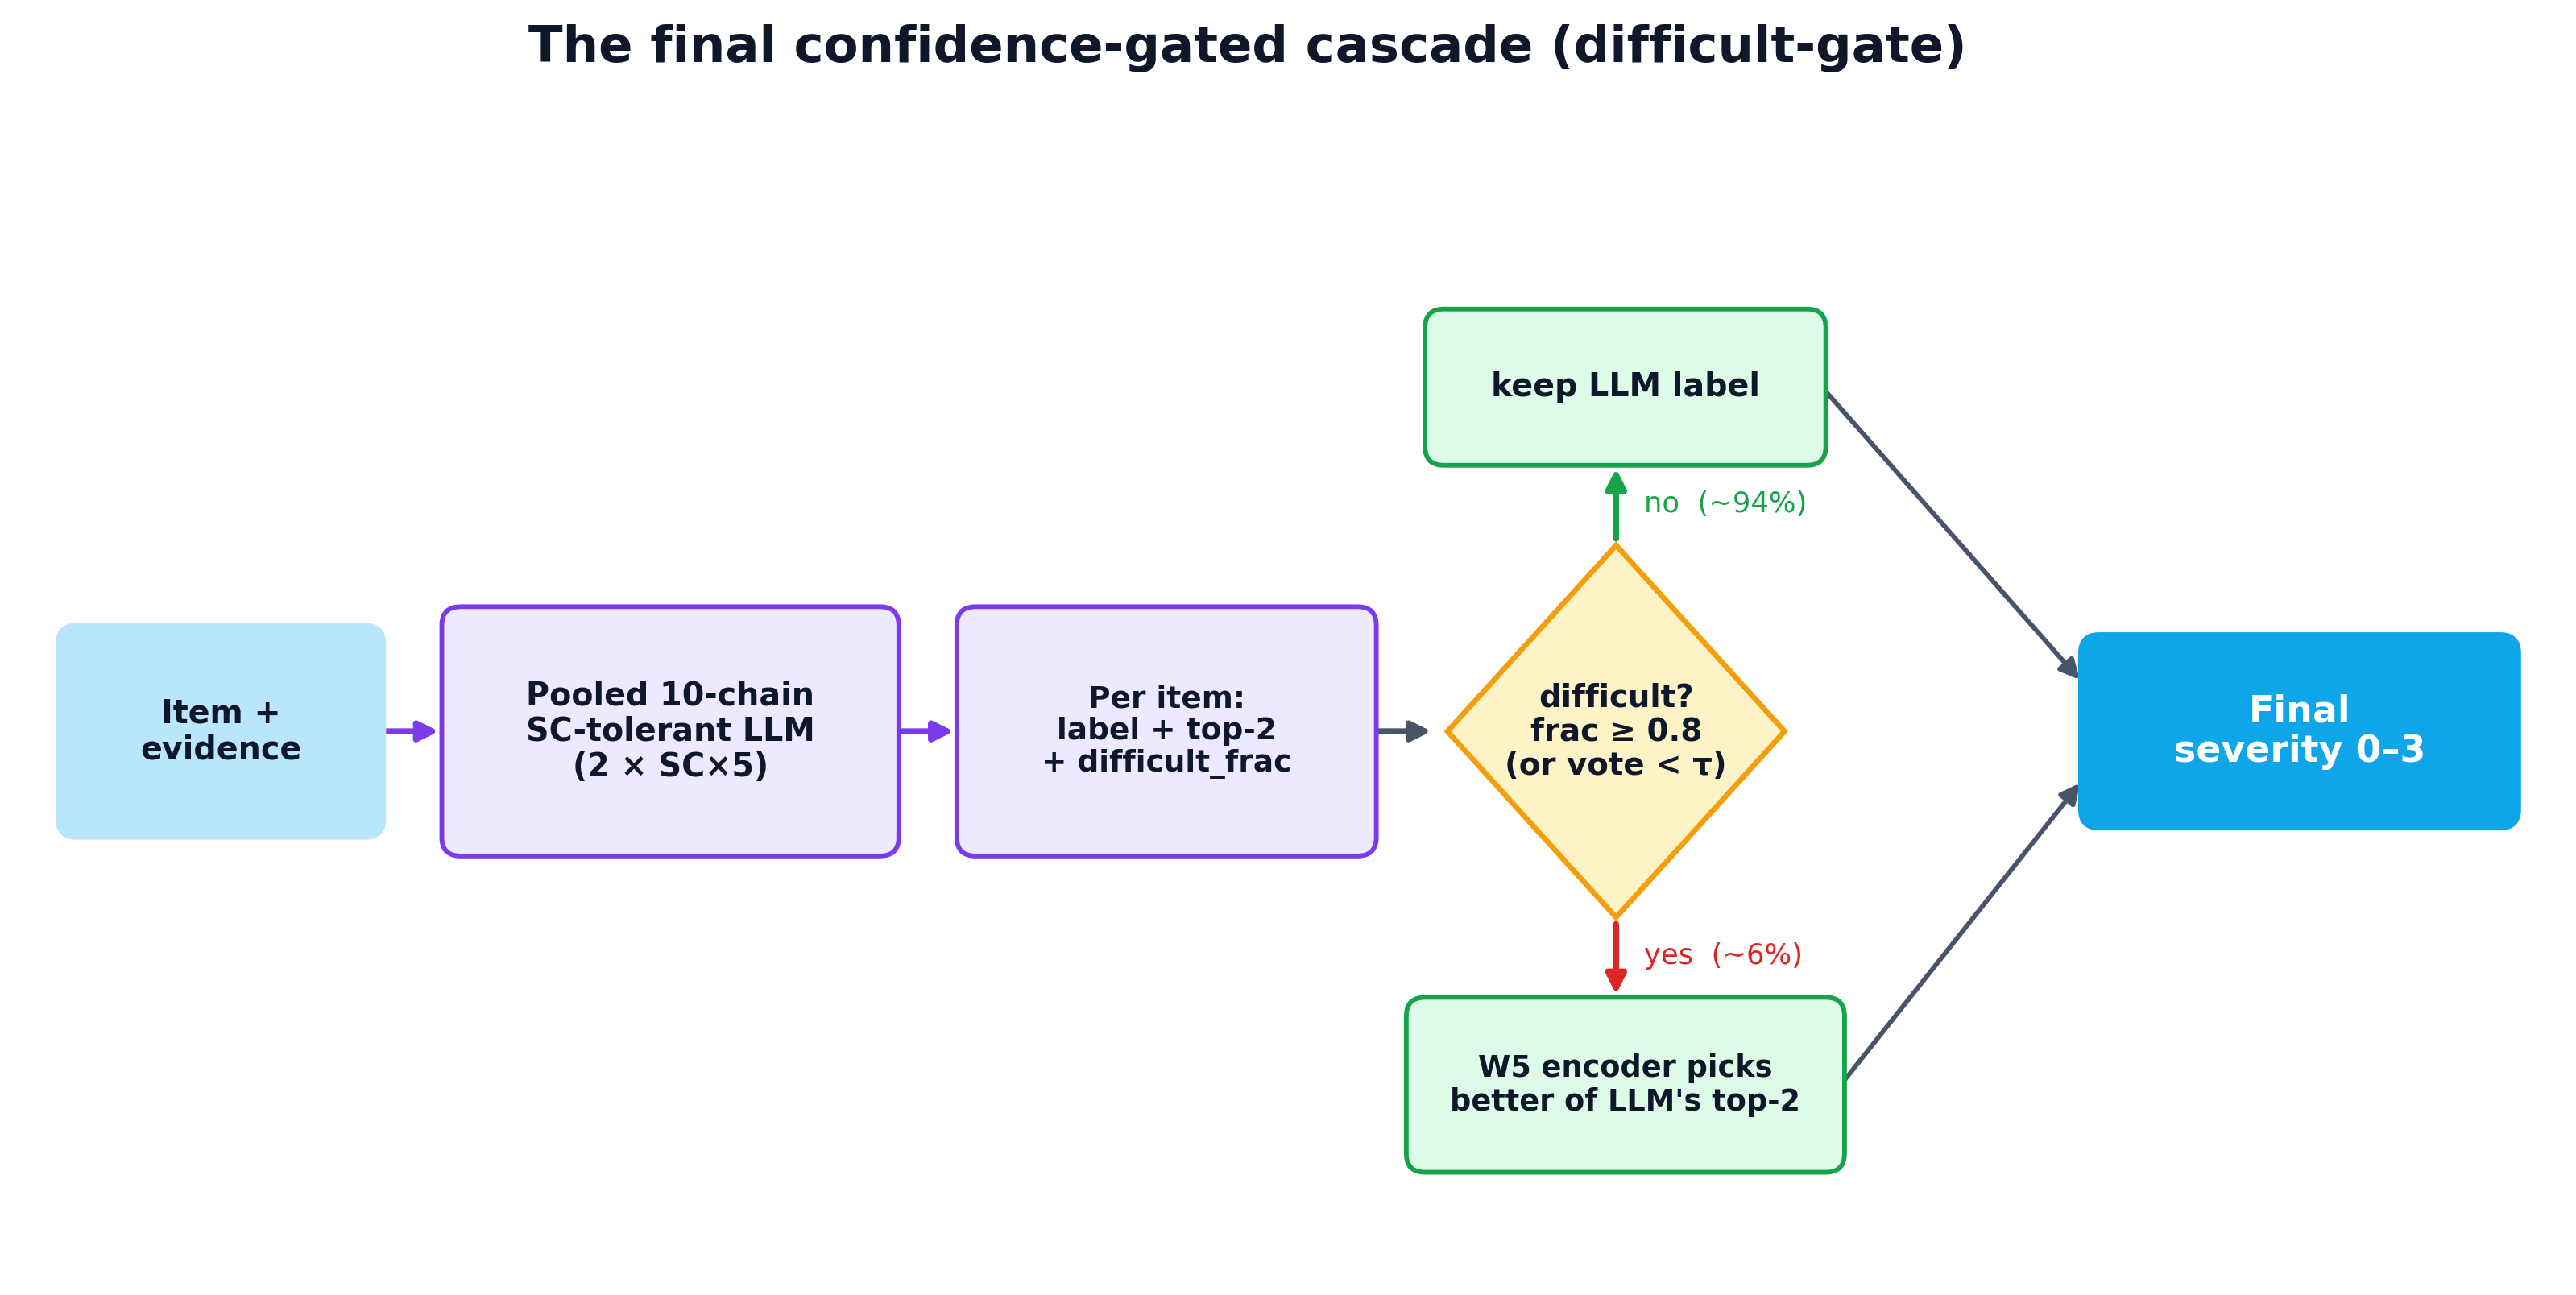
\includegraphics[width=\textwidth]{fig_arch_final_cascade.png}}
  \caption{End-to-end formulation. Each PHQ-8 item conditions participant-local retrieval; the selected evidence is scored by an ordinal encoder and an LLM reasoning model, while evidence status and uncertainty determine training and selective correction. \rev{Interim rendering from the project archive; the final vector version of this figure still has to be produced.}}
  \label{fig:pipeline}
\end{figure*}

\section{Results}
\label{sec:results}

\subsection{Retrieval-Conditioned Ordinal Baseline}
\label{subsec:baseline-results}
Table~\ref{tab:baseline} summarizes the matched retrieval and encoder comparisons that established the baseline. Context windows improved over a single BM25 utterance, and hybrid retrieval generally produced stronger ordinal agreement. MentalBERT with Hybrid-W5 and CORN was the strongest standalone encoder in this phase, reaching macro-F1 0.372, QWK 0.390, and MAE 0.664. CORN also yielded the best balanced loss profile \del{for this evidence/backbone setting}\rev{for MentalBERT with Hybrid-W5}: plain and weighted cross-entropy reached macro-F1 0.358 and 0.357, compared with 0.372 for CORN\rev{; for BERT-base the ordering reverses (CORN 0.325 versus plain cross-entropy 0.340), so the advantage of the ordinal loss is backbone-specific}. \rev{A five-seed replication of the Hybrid-W3 backbone comparison (seeds 42, 7, 31, 123, 2024) showed modest seed sensitivity---MentalBERT macro-F1 $0.350\pm0.005$ and QWK $0.357\pm0.010$---with MentalBERT beating BERT-base on all five seeds.} Later reasoning and evidence-quality experiments froze Hybrid-W3 as R0 so that changes in inference or query expansion could be measured against a fixed evidence condition.

\begin{table}[t]
  \caption{Matched participant-grouped OOF baselines with CORN and maximum length 256.}
  \label{tab:baseline}
  \centering
  \scriptsize
  \begin{tabular}{llrrrr}
    \toprule
    Backbone & Evidence & Macro-F1\rev{ $\uparrow$} & QWK\rev{ $\uparrow$} & MAE $\downarrow$ & F1$_3$\rev{ $\uparrow$} \\
    \midrule
    BERT & BM25 utterance & 0.274 & 0.119 & 0.847 & 0.093 \\
    BERT & Hybrid W3 & 0.348 & 0.336 & 0.740 & 0.185 \\
    MentalBERT & BM25 utterance & 0.299 & 0.220 & 0.744 & 0.060 \\
    MentalBERT & Hybrid W3 (R0) & 0.348 & 0.354 & 0.680 & 0.159 \\
    \best{MentalBERT} & \best{Hybrid W5} & \best{0.372} & \best{0.390} & \best{0.664} & \best{0.261} \\
    \bottomrule
  \end{tabular}
\end{table}

\subsection{Severity Compression and the Controlled Encoder--LLM Trade-off}
\label{subsec:reasoning-results}
The Hybrid-W3 MentalBERT+CORN encoder was exactly correct on 45.5\% of rows and off by one on a further 42.6\%; 88.1\% of predictions were therefore within one level. However, its class-wise F1 decreased from 0.589 for class 0 to 0.159 for class 3. Among true class-3 items, only 10.2\% were predicted as class 3. The model was ordinally conservative: large errors were uncommon, but severe symptoms were compressed toward the middle of the scale.

Replacing only the inference mechanism with per-item CoT changed this operating point. Macro-F1 increased from 0.348 to 0.373 and class-3 F1 from 0.159 to 0.295, but QWK fell from 0.354 to 0.312, MAE rose from 0.680 to 0.750, and far-off errors increased from 0.119 to 0.180. The LLM was more willing to predict severe symptoms, but also more likely to make extreme unsupported calls. The two models agreed on 44.7\% of rows. In disagreements, only the encoder was correct on 327 examples and only the CoT model on 380; for true class 3, the corresponding counts were 6 and 38. This establishes complementarity at the example level rather than a simple average-metric advantage.

\begin{figure*}[t]
  \centering
  \IfFileExists{final_report_fig2_reasoning_tradeoff.pdf}{%
    \includegraphics[width=\textwidth]{final_report_fig2_reasoning_tradeoff.pdf}%
  }{\includegraphics[width=\textwidth]{fig16_cot_vs_mbert_hybw3.png}}
  \caption{Controlled comparison on the same Hybrid-W3 evidence. The LLM recovers more severe items, whereas the encoder maintains a safer ordinal error profile. \rev{Interim rendering from the project archive; the final vector version of this figure still has to be produced.}}
  \label{fig:reasoning-tradeoff}
\end{figure*}

\subsection{Cross-Item Reasoning, Self-Consistency, and Selective Correction}
\label{subsec:cascade-results}
Allowing unrestricted cross-item context did not improve the result. Joint CoT obtained macro-F1 0.339, QWK 0.334, MAE 0.727, and class-3 F1 0.163. Qualitative inspection showed a clinical-halo failure mode: evidence of general depression elevated weakly supported item scores. Staging the information flow improved macro-F1 to 0.355, QWK to 0.352, and MAE to 0.686, but reduced class-3 F1 to 0.130, indicating excessive caution. These variants demonstrate that the prompt objective controls the balance between cross-symptom over-attribution and severe under-calling.
% VERIFIED 2026-07-16: Joint/Staged metrics were recomputed directly from the five
% OOF fold files (outputs/cot/folds_joint/, outputs/cot/folds_staged/); they match
% the values above at printed precision (Joint 0.3394/0.3341/0.7272/0.1627,
% Staged 0.3551/0.3520/0.6855/0.1300). Source check resolved.

The tolerance-aware staged prompt combined with pooled self-consistency provided a more balanced LLM parent: macro-F1 0.400, QWK 0.406, MAE 0.641, exact accuracy 0.513, and far-off rate 0.128. Table~\ref{tab:models} compares this parent with the main encoders and cascades. The difficult-only gate routed 5.9\% of rows, too few for the correction branch to materially change performance. The merged gate routed 41.5\%. With Attention-MIL as the correction expert, it achieved the best pre-R2 overall profile: macro-F1 0.409, QWK 0.447, MAE 0.606, accuracy 0.530, and far-off rate 0.118. Rerank+CORN yielded the lowest far-off rate, 0.115, but lower macro-F1 and QWK. Thus, Attention-MIL was most useful not as a standalone classifier but as a narrow expert for uncertain, top-two decisions.

\begin{table*}[t]
  \caption{Model and cascade comparison on aligned Hybrid-W3 OOF predictions. The LLM is the pooled 10-chain tolerance-aware model. \rev{The bolded row marks the selected overall configuration; in the far-off column, bold marks the column best (Rerank+CORN).}}
  \label{tab:models}
  \centering
  \scriptsize
  \begin{tabular}{lrrrrrr}
    \toprule
    Configuration & Accuracy\rev{ $\uparrow$} & Macro-F1\rev{ $\uparrow$} & QWK\rev{ $\uparrow$} & MAE $\downarrow$ & Far-off $\downarrow$ & Routed \\
    \midrule
    MentalBERT+CORN encoder & 0.455 & 0.348 & 0.354 & 0.680 & 0.119 & -- \\
    Attention-MIL encoder & 0.475 & 0.360 & 0.362 & 0.671 & 0.130 & -- \\
    Pooled tolerance-aware LLM & 0.513 & 0.400 & 0.406 & 0.641 & 0.128 & -- \\
    Attention-MIL difficult-gate cascade & 0.519 & 0.402 & 0.417 & 0.635 & 0.130 & 5.9\% \\
    % Revision: 0.118 un-bolded -- it is not the far-off column best (0.115 below is).
    \best{Attention-MIL merged-gate cascade} & \best{0.530} & \best{0.409} & \best{0.447} & \best{0.606} & 0.118 & 41.5\% \\
    Rerank+CORN merged-gate cascade & 0.511 & 0.394 & 0.411 & 0.627 & \best{0.115} & 41.5\% \\
    \bottomrule
  \end{tabular}
\end{table*}

\subsection{Evidence Quality, Retrieval Expansion, and Missing Evidence}
\label{subsec:evidence-results}
A lexical hit does not imply usable symptom evidence. In the frozen Hybrid-W3 audit, the NoInterest lexicon matched 99.5\% of participant-level evidence sets, whereas a binary LLM audit judged only 2.3\% to contain relevant support. The corresponding keyword-versus-judged rates were 63.9\% versus 0.9\% for Moving, 56.6\% versus 4.6\% for Appetite, and 54.8\% versus 3.7\% for Concentrating. This motivated replacing hit rate with the four-way evidence judge.

The label-free R1 selection produced only a modest average change in judged informativeness: 0.287 for R0 versus 0.294 for R1\rev{; the diagnostic BM25-only expanded variant scored 0.269 and the both-sides expansion 0.293}. Gains were concentrated in Concentrating (+0.036), NoInterest (+0.027), Moving (+0.018), and Appetite (+0.014), while Failure and Tired \rev{(and, marginally, Sleep)} declined. The standalone MentalBERT+CORN encoder improved from macro-F1 \del{0.347}\rev{0.348} to 0.372, QWK 0.354 to 0.384, and class-3 F1 0.159 to 0.223. However, participant-cluster bootstrap intervals included zero for macro-F1, QWK, and MAE, so these changes are suggestive rather than statistically established. The LLM gained 0.010 macro-F1 but lost QWK and MAE, and the frozen merged cascade regressed from QWK 0.447 to 0.410 and MAE 0.606 to 0.640. The cascade MAE regression was the only \rev{macro-F1, QWK, or MAE} R1--R0 interval among these headline comparisons that excluded zero\rev{; in the same analysis, the cascade accuracy delta ($[-0.052,-0.001]$) and the standalone Attention-MIL far-off delta ($[-0.043,-0.008]$) also excluded zero}.

The clearest R1 result came from treating judged-none training rows as missing. As shown in Table~\ref{tab:evidence}, \del{loss masking did not improve the status quo}\rev{loss masking traded slightly worse macro-F1 and QWK for the best class-3 F1 among the three policies (0.242 versus 0.223 for the status quo), at the cost of the highest false-severe rate (0.028)}, whereas dropping judged-none training pairs increased encoder macro-F1 to 0.393, QWK to 0.421, and class-3 recall to 0.192, while reducing MAE to 0.645. This came with a small increase in false-severe predictions, from 0.020 to 0.024. Because \texttt{drop} changes the effective label distribution, the R2 analysis must report removals by item and gold class before interpreting the gain.

\begin{figure*}[t]
  \centering
  \IfFileExists{final_report_fig3_evidence.pdf}{%
    \includegraphics[width=\textwidth]{final_report_fig3_evidence.pdf}%
  }{%
    \begin{minipage}[c]{0.49\textwidth}\centering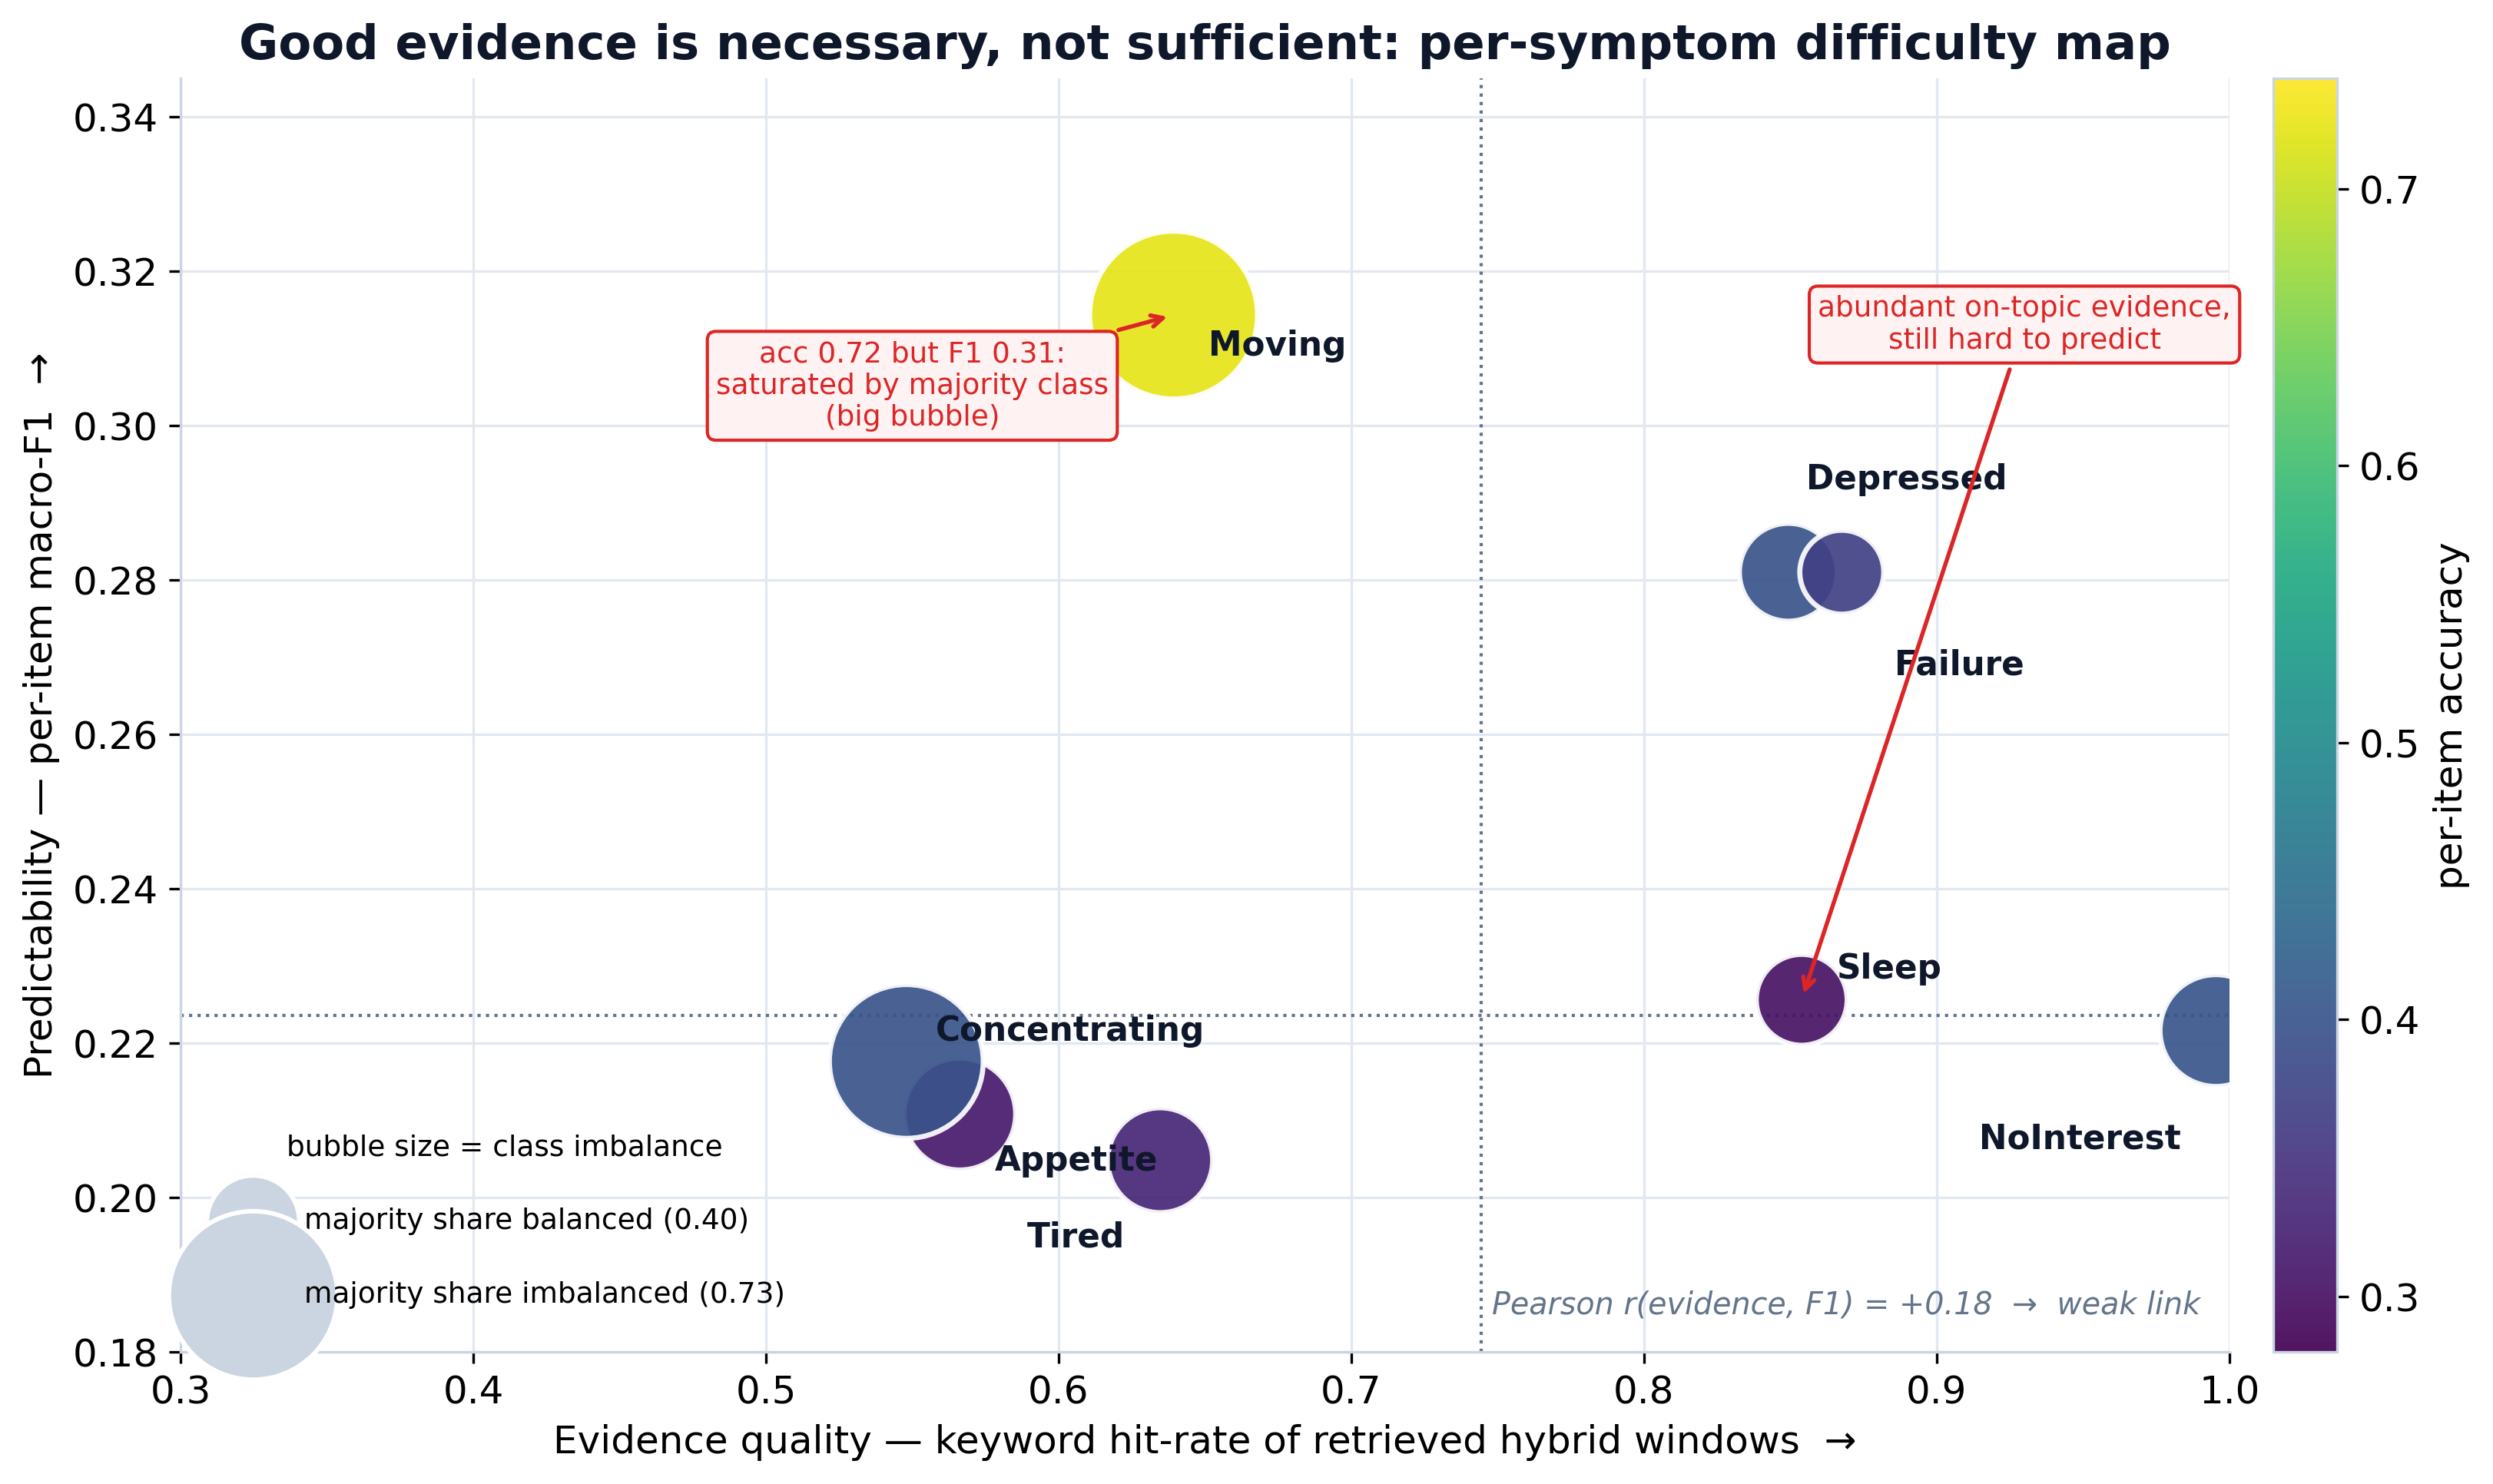
\includegraphics[width=\linewidth]{fig3_evidence_quality_map.png}\end{minipage}\hfill
    \begin{minipage}[c]{0.49\textwidth}\centering\includegraphics[width=\linewidth]{fig3b_retrieval_trajectory.png}\end{minipage}}
  \caption{Lexical coverage is not equivalent to usable symptom evidence. Panel A contrasts keyword coverage with judged evidence; Panel B tracks per-item evidence quality and downstream predictability from R0 to R1\del{, with R2 added only after validation}\rev{. The R2 selection is now validated (informative rate 0.307, Section~\ref{subsec:r2-results}) and must be added to Panel B when the final figure is produced; the interim panels shown are the archived project figures.}}
  \label{fig:evidence-quality}
\end{figure*}

\begin{table*}[t]
  \caption{Effect of expanded retrieval and missing-evidence policies. R1 policies are applied only to encoder training folds; validation and OOF rows remain unchanged. \del{Dashes indicate metrics not reported in the current policy summary.}\rev{Bold marks the best encoder training policy; the LLM and cascade blocks are aligned reference points, not policy candidates.}}
  \label{tab:evidence}
  \centering
  \scriptsize
  \begin{tabular}{llrrrrrr}
    \toprule
    Model & Retrieval/policy & Macro-F1\rev{ $\uparrow$} & QWK\rev{ $\uparrow$} & MAE $\downarrow$ & F1$_3$\rev{ $\uparrow$} & Recall$_3$\rev{ $\uparrow$} & Far-off $\downarrow$ \\
    \midrule
    MentalBERT+CORN & R0 Hybrid-W3 & \rev{0.348} & 0.354 & 0.680 & 0.159 & 0.102 & 0.119 \\
    MentalBERT+CORN & R1, zero/status quo & 0.372 & 0.384 & 0.671 & 0.223 & 0.150 & 0.123 \\
    MentalBERT+CORN & R1, mask & 0.364 & 0.371 & 0.684 & \rev{0.242} & 0.174 & 0.130 \\
    \best{MentalBERT+CORN} & \best{R1, drop} & \best{0.393} & \best{0.421} & \best{0.645} & \rev{\textbf{0.270}} & \best{0.192} & 0.120 \\
    \midrule
    LLM only & R0 & 0.400 & 0.406 & 0.641 & 0.254 & 0.204 & 0.128 \\
    LLM only & R1 & 0.410 & 0.397 & 0.653 & 0.269 & 0.222 & 0.134 \\
    MIL merged cascade & R0 & 0.409 & 0.447 & 0.606 & 0.256 & 0.198 & 0.118 \\
    MIL merged cascade & R1 & 0.405 & 0.410 & 0.640 & 0.266 & 0.210 & 0.120 \\
    \bottomrule
  \end{tabular}
\end{table*}

{\color{red}% ---- New subsection: completed R2 results (replaces the former R2 TODO) ----
\subsection{Systematic Retrieval Study (R2)}
\label{subsec:r2-results}
The four-lexicon ablation contradicted the expansion hypothesis. Under the revised judge, the best top-5 configuration per lexicon was the frozen core vocabulary (set informative rate 0.316, obtained by $\alpha=0.25$ fusion), core+clinical with BM25 (0.295), the full expansion with semantic retrieval (0.295), and core+lay with semantic retrieval (0.293): no expansion tier beat the unexpanded core. The two single retrievers are complementary at the example level---among core-lexicon top-5 sets, BM25 was uniquely informative for 150 participant--items and semantic retrieval for 192, with 345 informative under both---so a fusion sweep over $\alpha\in\{0.25,0.5,0.75\}$ was triggered and judged. Selecting across evidence budgets with the pre-registered hierarchy (highest informative rate; 0.005 ties broken by lower none, then ambiguous, then redundancy rate, then fewer windows, then the simpler retriever), the semantic-weighted $\alpha=0.25$ fusion with a top-3 budget maximized judged informative rate at \best{0.327} and was the \emph{sole} candidate inside the 0.005 tolerance band (next best 0.316). It therefore beat both single retrievers---semantic top-5 at 0.307 and semantic top-3 at 0.312---by more than the 0.005 margin and was selected as R2, overturning the provisional semantic-only choice. A verification confirmed each fused set was judged on its own HybridScore ranking rather than a union: only 0.9\% of selected top-3 sets equal the BM25$\cup$semantic top-3 union, and 45.5\% contain a window promoted into the top three from outside both single-retriever top-3 lists.

Downstream, the prediction study was re-run from scratch on the selected fused ($\alpha=0.25$, top-3) evidence---the encoder under the three missing-evidence training policies, the Qwen predictor under the five evidence conditions, and both leakage-safe cascades---and the provisional numbers obtained on the superseded semantic-only R2 are intentionally not carried over. At the time of writing the encoder out-of-fold predictions have completed and the Qwen conditions are still generating, so Table~\ref{tab:r2} reports the configuration and constraint structure with the final fused-evidence numbers pending. The constrained-selection logic is unchanged from the pre-registration: the encoder policy is chosen by best constraint-passing QWK under an explicit false-severe allowance ($+0.015$ over status quo) and an MAE ceiling; the LLM condition by best constraint-passing QWK under an MAE ceiling; and a leakage-safe cascade is accepted only if it exceeds its better single component, with routing thresholds fit inside training folds rather than on the OOF. The frozen R0 merged-gate cascade (QWK 0.447, macro-F1 0.409, MAE 0.606) remains the reference best system pending the refreshed comparison.

\begin{table*}[t]
  \caption{\color{red}R2 systematic study, downstream constrained selection on the fused $\alpha=0.25$/top-3 evidence (participant-grouped OOF, 1{,}752 rows). \emph{Numbers pending}: the encoder policies, the Qwen conditions, and the two leakage-safe cascades are being recomputed on the fused evidence (encoder OOF complete; Qwen array still running). The provisional semantic-R2 numbers are intentionally omitted rather than reused. The frozen R0 cascade is a fixed reference.}
  \label{tab:r2}
  \centering
  \scriptsize
  \color{red}
  \begin{tabular}{llrrrrr}
    \toprule
    Configuration & Status & QWK $\uparrow$ & Macro-F1 $\uparrow$ & MAE $\downarrow$ & Recall$_3$ $\uparrow$ & False-severe $\downarrow$ \\
    \midrule
    R2 encoder, status quo & \todoRtwo{pending} & -- & -- & -- & -- & -- \\
    R2 encoder, mask & \todoRtwo{pending} & -- & -- & -- & -- & -- \\
    R2 encoder, drop & \todoRtwo{pending} & -- & -- & -- & -- & -- \\
    R2 LLM, keep-all & \todoRtwo{pending} & -- & -- & -- & -- & -- \\
    R2 LLM, filter/info-first/fallback/long-ctx & \todoRtwo{pending} & -- & -- & -- & -- & -- \\
    R2 cascade, encoder-first / LLM-first & \todoRtwo{pending} & -- & -- & -- & -- & -- \\
    \midrule
    Frozen R0 MIL merged cascade & reference (best overall) & 0.447 & 0.409 & 0.606 & 0.198 & -- \\
    \bottomrule
  \end{tabular}
\end{table*}
}%
\todoRtwo{Downstream refresh in progress: populate Table~\ref{tab:r2} and the prose above from the fused $\alpha=0.25$/top-3 evidence once the encoder metrics and the Qwen L1--L5 array complete (jobs \texttt{19405517} done, \texttt{19405519} running); do not reuse the superseded semantic-R2 downstream numbers.}

\subsection{Per-Item and Severe-Class Analysis}
\label{subsec:item-results}
Performance remains heterogeneous across symptoms. Under R1, the weakest encoder items were NoInterest (macro-F1 0.28), Moving (0.32), Concentrating (0.33), and Tired (0.36). Depressed and Sleep have relatively direct linguistic expressions and high judged informative rates, whereas NoInterest is often expressed through reduced activities or social withdrawal rather than the literal phrase ``no interest.'' Moving corresponds to psychomotor slowing or agitation, information that may be expressed through timing, voice, or visible behavior rather than lexical content, making it a structural limitation of text-only prediction. Explicit lexical matches were associated with accuracy 0.42 \rev{($n=287$)}, compared with 0.36 when the judge found supporting evidence without a lexicon hit \rev{(only $n=14$ such rows, so this contrast is anecdotal)}, consistent with greater difficulty for indirect descriptions. Severe under-calling remained prominent: in the R1 encoder, 55\% of true class-3 items were predicted at 0 or 1.

\section{Discussion}
\label{sec:discussion}
The experiments support a decomposition of item-level depression prediction into evidence selection, severity inference, and uncertainty-aware model selection. Hybrid retrieval improved the initial encoder, but later evidence audits showed why retrieval metrics must be interpreted cautiously. Query expansion increased the probability of lexical contact with a symptom, yet only small changes were observed in judged informativeness. In particular, the BM25-only expanded variant performed worse than the frozen hybrid on the evidence judge \rev{(informative rate 0.269 versus 0.287)}, demonstrating that term coverage is not a sufficient retrieval objective. \del{The R2 study therefore tests BM25 and semantic retrieval independently before deciding whether fusion is justified.} \rev{The R2 study tested BM25 and semantic retrieval independently and confirmed the pattern: no lexicon expansion improved judged evidence quality. The two-sided unique wins (150 BM25-only versus 192 semantic-only informative sets) justified testing calibrated fusion, and the judged $\alpha$-sweep confirmed fusion helps: the semantic-weighted $\alpha=0.25$ combination with a top-3 budget beat every single-retriever configuration on judged evidence quality (informative rate 0.327 versus 0.307 for semantic-only) and was selected as R2. The preferred evidence selector is thus a semantic-dominant retriever with a light BM25 component, not term expansion.}

The encoder and LLM occupy different points on a severity--safety trade-off. CORN and class imbalance encourage a stable middle-of-scale predictor: most errors remain adjacent, but severe items are compressed. Explicit LLM reasoning is more willing to infer severe symptoms and recovers many examples missed by the encoder, but it can also over-attribute a symptom from generic distress or cross-item context. Joint reasoning exposed this clinical-halo failure mode, while staged and tolerance-aware prompts showed that constraining information flow and the stated objective can substantially change the error distribution without changing the model or evidence.

Selective correction was valuable because the models failed on different examples. The best cascade did not simply average their predictions; it retained broad LLM reasoning and used an encoder only on uncertain items, restricted to the LLM's top two classes. Attention-MIL was effective in this narrow role even though it was not the best standalone predictor. However, the R1 result also shows that a frozen gate may not transfer when retrieval changes. The negative R1 cascade result should therefore not be interpreted as evidence that better retrieval cannot help a cascade; rather, the input distribution changed while the routing rule remained fixed. \rev{On the superseded semantic-only R2 evidence, neither leakage-safe cascade beat its better single component even with routing refit inside training folds, suggesting cascade gains are tied to the specific complementarity profile of the R0 components rather than to selective correction in general; whether this persists under the selected fused ($\alpha=0.25$/top-3) evidence is being re-evaluated (Table~\ref{tab:r2}, pending).}

The \texttt{drop} result highlights a fundamental label--evidence mismatch. A participant may endorse a PHQ symptom on the questionnaire without discussing it in the interview. Training a text classifier on such a row asks it to infer a label from absent information. Removing judged-none rows improved the encoder more than query expansion alone, but this result depends on the accuracy of a model-based judge and may alter class and item distributions. \del{The systematic experiment must therefore audit which rows are removed and use an independent judge model to reduce circularity with the Qwen predictor.} \rev{The systematic R2 experiment audited the removals and enforced an explicit false-severe constraint on encoder-policy selection; on the superseded semantic-only evidence \texttt{drop} was rejected despite the best raw QWK because its false-severe rate exceeded the pre-registered $+0.015$ allowance, and this constrained selection is being repeated on the fused evidence (Table~\ref{tab:r2}, pending). The attempt to substitute an independent judge failed---MentaLLaMA-chat-7B/13B produced degenerate judgments---so judge--predictor circularity persists, and the drop-versus-status-quo question should be revisited once a validated independent judge is available.}

Several limitations constrain the claims. The study uses 219 participants from one corpus and internal participant-grouped OOF evaluation, not an external clinical cohort. Severe labels are rare, several experiments use a single training seed \rev{(although a five-seed replication of the backbone comparison bounded seed variability at roughly $\pm 0.005$--$0.010$ macro-F1/QWK)}, and the evidence judge has not been validated against a large clinician-annotated set \rev{and shares a model family with the LLM predictor}. Speaker roles are not uniformly reliable, and text-only input omits acoustic and visual cues that are especially relevant to psychomotor behavior. Retrieved excerpts are candidate evidence, not causal explanations. Reconstructed PHQ totals and threshold metrics are internal diagnostics and do not establish screening utility. Finally, both missed severe symptoms and unsupported severe predictions are clinically consequential; any practical use would require explicit uncertainty, privacy safeguards, and human review.

\section{Conclusion}
\label{sec:conclusion}
We formulated PHQ-8 item prediction from mental-health interviews as an evidence-conditioned ordinal task. Contextual hybrid retrieval and MentalBERT+CORN provided a stable encoder baseline, while LLM reasoning recovered more severe cases at the cost of larger errors. Their complementary failure patterns enabled selective correction, and evidence-quality analysis showed that missing or irrelevant evidence remains a central bottleneck. The strongest completed evidence-aware intervention was to drop judged-none training pairs, while broad retrieval expansion produced only modest and statistically uncertain downstream gains. \rev{The systematic R2 study refined this picture: with a provenance-audited lexicon and stronger natural-language semantic queries, the frozen core vocabulary maximized judged evidence quality and expansion never helped, but a judged fusion sweep showed that a calibrated, semantic-weighted ($\alpha=0.25$) BM25--dense combination with a three-window budget is the best evidence selector, improving judged informative rate to 0.327 from 0.307 for semantic-only retrieval. The answer to the retrieval question is therefore that a well-queried, semantic-dominant retriever with a light lexical component---not term expansion---is the preferred evidence selector. The downstream re-evaluation of the encoder, LLM, and selective cascade on this fused evidence is in progress; until it completes, the frozen R0 merged-gate cascade remains the reference best system.} \todoRtwo{populate the R2 downstream numbers (Table~\ref{tab:r2}) once the fused-evidence encoder/LLM/cascade evaluations complete.}

{\color{red}% ---- New sections added in the revision pass ----
\section*{Ethics and Broader Impact}
This work analyzes interviews from people reporting depressive symptoms and predicts symptom severities; it is research on model behavior, not a diagnostic instrument. Both error directions are clinically consequential: missed severe symptoms can delay care, while unsupported severe predictions can stigmatize or trigger unwarranted intervention---our false-severe constraint in R2 is a first, not sufficient, mitigation. Retrieved excerpts are candidate evidence, not clinical rationales, and could mislead a reviewer if presented as explanations. Any downstream use would require clinician oversight, calibrated uncertainty, and consent-respecting handling of interview data; the transcripts contain sensitive personal disclosures and must not be redistributed. We do not release model outputs linked to identifiable participants.

\section*{Data and Code Availability}
E-DAIC is available from USC ICT under a license agreement; we redistribute no transcripts or labels. All code, SLURM run scripts, frozen retrieval artifacts, and OOF prediction files reproducing every number in this paper are available in the project repository; the context-window banks are included as data artifacts (the bank-builder script is not part of the release, as noted in Section~\ref{subsec:retrieval}).
}

\bibliographystyle{unsrt}
\bibliography{references_working_v2}

\end{document}
